\addcontentsline{toc}{chapter}{LAMPIRAN}
\appendix 
\chapter{Perbandingan Fitur Sistem \textit{Tracer Study}}

\begin{figure}[H]
	\centering
	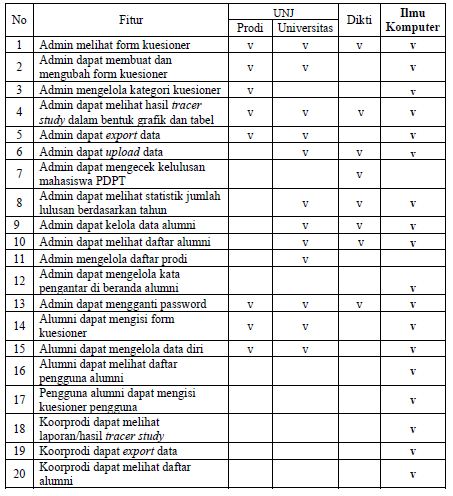
\includegraphics[width=1.0\textwidth]{gambar/tabelFitur}
	\label{tabelFitur}
\end{figure}

\begin{figure}[H]
	\centering
	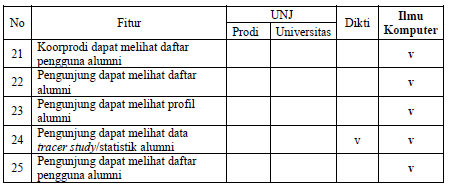
\includegraphics[width=1.0\textwidth]{gambar/tabelFitur2}
	\label{tabelFitur2}
\end{figure}

\chapter{Perbandingan Kuesioner Sistem \textit{Tracer Study}}

\begin{figure}[H]
	\centering
	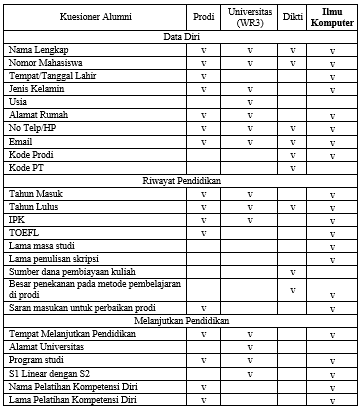
\includegraphics[width=1.0\textwidth]{gambar/tabelKuesioner}
	\label{tabelKuesioner}
\end{figure}

\begin{figure}[H]
	\centering
	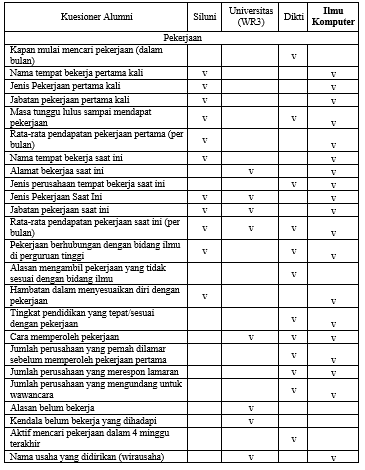
\includegraphics[width=1.0\textwidth]{gambar/tabelKuesioner2}
	\label{tabelKuesioner2}
\end{figure}

\begin{figure}[H]
	\centering
	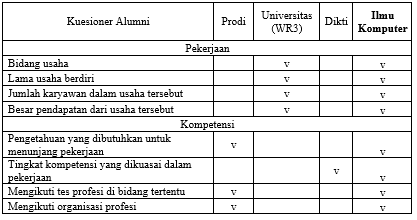
\includegraphics[width=1.0\textwidth]{gambar/tabelKuesioner3}
	\label{tabelKuesioner3}
\end{figure}

\chapter{Analisis Kebutuhan Sistem dengan Pihak Prodi Ilmu Komputer}

\begin{enumerate}
	\item Kapan diadakannya kegiatan tracer study pada prodi Ilmu Komputer?
	Kegiatan tracer study telah dilakukan sejak prodi ini memiliki lulusan pertama pada semester 2016/2017.
	\item Bagaimana proses pelaksanaan tracer study pada prodi Ilmu Komputer?
	Pelaksanaan tracer study tersebut dilakukan melalui pengiriman kuesioner melalui pos, e-mail dan media sosial seperti whatsapp
	\item Apakah terdapat kendala selama proses tracer study berlangsung?
	Bentuk pelaksanaan tersebut dirasa kurang efektif karena dapat membutuhkan waktu lama terhadap respon alumni
	\item Apakah saat ini sudah tersedia sistem tracer study yang dapat diakses secara online?
	Saat ini terdapat sistem tracer study milik WR3 yang juga memiliki layanan di tingkat prodi. Karena sistem yang disediakan bersifat umum untuk semua prodi terdapat beberapa kebutuhan dari prodi Ilkom yang belum bisa dipenuhi sistem tersebut seperti belum ada pengisian kuesioner oleh pengguna lulusan/alumni.  Selain itu, juga terdapat sistem tracer study milik Dikti namun untuk tingkat perguruan tinggi. 
	\item Mengapa diperlukan kuesioner untuk pengguna alumni?
	Penelitian terhadap pengguna diperlukan untuk mengetahui bagaimana penilaian pengguna terhadap kompetensi lulusan dan kurikulum yang berjalan apakah sudah mencukupi dan relevan dengan kebutuhan dunia kerja saat ini. 
	\item Jika akan dilakukan pengembangan sistem tracer study dikhususkan untuk prodi Ilmu Komputer, fasilitas apa yang diharapkan dari pengembangan sistem ini?
	\begin{itemize}
		\item Selain kuesioner untuk alumni juga disediakan fitur pengisian kuesioner secara online untuk pengguna alumni
		\item Koorprodi membutuhkan akses ke sistem untuk mengakses data tracer yang diperlukan bagi akreditasi maupun penjaminan mutu internal
		\item Disediakan open access bagi pengunjung untuk dapat melihat beberapa hasil tracer study seperti yang terdapat pada sistem tracer study Dikti. 
		\item Bandingkan sistem tracer study UNJ dan Dikti, ambil fitur yang sekiranya dapat bermanfaat untuk prodi. 
	\end{itemize}	
\end{enumerate}
\vspace{0.8cm}

\begin{tabular}{p{7.5cm}c}
	&Jakarta, April 2019\\
	&\\
	&\\
	&\\
	&\textbf{Ir. Fariani Hermin Indiyah, M.T}
\end{tabular}

\chapter{Sampel Kode \textit{Controller} Alumni pada Admin}

\begin{verbatim}

<?php
defined('BASEPATH') OR exit('No direct script access allowed');

class Alumni extends CI_Controller {
function __construct(){
parent::__construct();
if($_SESSION["logged_in"] != 'login') {
redirect(base_url("login"));
}

$this->load->model('m_alumni');
$this->load->model('m_master');
$this->load->model('m_pengguna');
$this->load->library(array('PHPExcel','PHPExcel/IOFactory'));

}

public function index()
{
$prodiID = $this->session->userdata('prodiID');
$data = array(
'role' => $this->session->userdata('role'),
'userID' => $this->session->userdata('userID'),
'prodiID' => $prodiID,
'alumni' => $this->m_alumni->getAlumni($prodiID),
);
$this->load->view('element/head');
$this->load->view('element/header');
$this->load->view('element/navbar', $data);
$this->load->view('admin/v_dataAlumni', $data);
$this->load->view('element/footer');
}

function exeAddAlumni()
{

$userID = 'ALU'.$this->input->post('nim');
$cek = $this->m_alumni->cekAlumni($this->input->post('nim'));

if($cek->num_rows() > 0){
$this->session->set_flashdata("gagalAddAlumni", '<div><div class="alert alert-danger" id="alert" align="center">Gagal menambahkan! Akun alumni sudah terdaftar</div></div>');
} else {

$data_user = array(
'userID' => $userID,
'username' => $this->input->post('nim'),
'password' => $this->input->post('nim'),
'prodiID' => $this->session->userdata('prodiID'),
'role' => 'alumni'
);
$this->m_master->inputData($data_user,'user');

$data_alumni = array(
'nama' => $this->input->post('nama'),
'nim' => $this->input->post('nim'),
'userID' => $userID,
'jenis_kelamin' => $this->input->post('jenis_kelamin'),
'tahun_masuk' => $this->input->post('tahun_masuk'),
'tahun_lulus' => $this->input->post('tahun_lulus'),
'prodiID' => $this->session->userdata('prodiID'),
);

$this->m_master->inputData($data_alumni,'alumni');

$this->session->set_flashdata("suksesAddAlumni", '<div><div class="alert alert-success" id="alert" align="center">Akun alumni berhasil ditambahkan!</div></div>');
}

redirect('admin/Alumni');
}

public function editProfil($id)
{
$data = array(
'role' => $this->session->userdata('role'),
'userID' => $this->session->userdata('userID'),
'prodiID' => $this->session->userdata('prodiID'),
'profil' => $this->m_alumni->getAlumniByID($id)
);
$this->load->view('element/head');
$this->load->view('element/header');
$this->load->view('element/navbar', $data);
$this->load->view('admin/v_editProfilAlumni', $data);
$this->load->view('element/footer');
}

function exeEditProfil()
{

$data_user = array(
'username' => $this->input->post('nim')
);
$id = $this->input->post('id');
$where = array('id' => $this->input->post('userID'));
$this->m_master->updateData($where,$data_user,'user');

$data_alumni = array(
'nama' => $this->input->post('nama'),
'nim' => $this->input->post('nim'),
'jenis_kelamin' => $this->input->post('jenis_kelamin'),
'tahun_masuk' => $this->input->post('tahun_masuk'),
'tahun_lulus' => $this->input->post('tahun_lulus'),
'ipk' => $this->input->post('ipk'),
'toefl' => $this->input->post('toefl'),
'alamat' => $this->input->post('alamat'),
'tempat_lahir' => $this->input->post('tempat_lahir'),
'tanggal_lahir' => $this->input->post('tanggal_lahir'),
'email' => $this->input->post('email'),
'no_telepon' => $this->input->post('no_telepon'),
);

$where = array('id' => $this->input->post('id'));
$this->m_master->updateData($where,$data_alumni,'alumni');

$this->session->set_flashdata("pesan", '<div><div class="alert alert-success" id="alert" align="center">Edit data alumni sukses!</div></div>');
redirect('admin/Alumni/editProfil/'.$id);
}

function exeImport()
{
if ($_FILES['file']['name']) {
$fileName = time().$_FILES['file']['name'];

$config['upload_path'] = FCPATH .'/assets/upload/';
$config['file_name'] = $fileName;
$config['allowed_types'] = 'xls|xlsx|csv';
$config['max_size'] = 10000;

$this->load->library('upload');
$this->upload->initialize($config);

if(! $this->upload->do_upload('file') )
$this->upload->display_errors();

$media = $this->upload->data('file');
$inputFileName = $this->upload->data('full_path');

try {
$inputFileType = IOFactory::identify($inputFileName);
$objReader = IOFactory::createReader($inputFileType);
$objPHPExcel = $objReader->load($inputFileName);
} catch(Exception $e) {
die('Error loading file "'.pathinfo($inputFileName,PATHINFO_BASENAME).'": '.$e->getMessage());
}

$sheet = $objPHPExcel->getSheet(0);
$highestRow = $sheet->getHighestRow();
$highestColumn = $sheet->getHighestColumn();

for ($row = 2; $row <= $highestRow; $row++){                  //  Read a row of data into an array
$rowData = $sheet->rangeToArray('A' . $row . ':' . $highestColumn . $row, NULL, TRUE, FALSE);

$nim = $rowData[0][1];
$cek = $this->m_alumni->cekAlumni($nim);
if($cek->num_rows() < 1){
//tabel user
$data = array(
"userID"=> "ALU".$rowData[0][1],
"username"=> $rowData[0][1],
"password"=> $rowData[0][1],
"role"=> 'alumni',
"prodiID" => $this->session->userdata('prodiID')
);

$insert = $this->db->insert("user",$data);
//tabel alumni
$data = array(
"nim"=> $rowData[0][1],
"nama"=> $rowData[0][0],
"no_telepon" => $rowData[0][2],
"ipk" => $rowData[0][3],
"userID"=> "ALU".$rowData[0][1],
"jenis_kelamin"=> $rowData[0][4],
"tahun_masuk"=> $rowData[0][5],
"tahun_lulus"=> $rowData[0][6],
"prodiID" => $this->session->userdata('prodiID')
);
$insert = $this->db->insert("alumni",$data);
} /*else {
unlink($inputFileName);
}*/
if ($rowData[0][7] != NULL) {
//tabel instansi
$where = array('nama_instansi' => $rowData[0][7]);
$cek = $this->m_master->cekData("instansi",$where)->num_rows();
if ($cek == 0) {
$data = array(
"nama_instansi" => $rowData[0][7],
"prodiID" => $this->session->userdata('prodiID')
);
$insert = $this->db->insert("instansi",$data);
$id_instansi = $this->m_master->getInstansiByName($rowData[0][7])->id;
} else {
$id_instansi = $this->m_master->getInstansiByName($rowData[0][7])->id;
}

//tabel pekerjaan
$alumniID = $this->m_alumni->getAlumniByUserID("ALU".$rowData[0][1])->id;
$where = array( 'id_alumni' => $alumniID);
$cek = $this->m_master->cekData("pekerjaan",$where)->num_rows();
if ($cek == 0) {
$firstPekerjaan = 'yes';
} else {
$firstPekerjaan = 'no';
}

$gajiawal = str_replace(".","",$rowData[0][9]);
$data = array(
"posisi" => $rowData[0][8],
"gaji" => $gajiawal,
"id_alumni" => $alumniID,
'firstPekerjaan' => $firstPekerjaan,
'id_instansi'=> $id_instansi
);
$insert = $this->db->insert("pekerjaan",$data);
} // if instansi not null

}
$this->session->set_flashdata("suksesImpor", '<div><div class="alert alert-info" id="alert" align="center">Data alumni berhasil diimpor</div></div>');
redirect('admin/Alumni');
} else {
$this->session->set_flashdata("gagalImpor", '<div><div class="alert alert-danger" id="alert" align="center">File belum dimasukkan</div></div>');
redirect('admin/Alumni');
}
}

function deleteAlumni($id){
//hapus pekerjaan
$where = array(
'id_alumni' => $id
);
$this->m_master->deleteData($where,'pekerjaan');
//hapus akun di tabel user
$userID = $this->m_alumni->getAlumniByID($id)->userID;
$where = array(
'userID' => $userID
);
$this->m_master->deleteData($where,'user');
//hapus data di tabel alumni
$where = array(
'id' => $id
);
$this->m_master->deleteData($where,'alumni');

$where = array(
'respondenID' => $id
);
$this->m_master->deleteData($where,'notif_kuesioner');
redirect('admin/Alumni');
}


}

\end{verbatim}


\chapter{Sampel Kode \textit{Model} Alumni pada Admin}

\begin{verbatim}

<?php 

class M_alumni extends CI_Model{	

public function __construct()
{
parent::__construct();
//$this->db2 = $this->load->database('db_dua', TRUE);
}

function getAlumniByUserID($userid)
{
$this->db->select('*');
$this->db->where('userID',$userid);
$query = $this->db->get('alumni');
return $query->row();

}

function getAlumniByID($id)
{
$this->db->select('*');
$this->db->where('id',$id);
$query = $this->db->get('alumni');
return $query->row();

}

function getAlumni($prodiID)
{
$this->db->select('*');
$this->db->where('status', 'aktif');
$this->db->where('prodiID', $prodiID);
$this->db->order_by('id', 'DESC');
$query = $this->db->get('alumni');
if($query->num_rows()>0)
{
return $query->result();
} else{
return $query->result();
}

}


function getAlumniByProdi($prodiID)
{
$this->db->select('*');
$this->db->where('status', 'aktif');
$this->db->where('prodiID', $prodiID);
$this->db->order_by('nama', 'ASC');
$query = $this->db->get('alumni');
if($query->num_rows()>0)
{
return $query->result();
} else{
return $query->result();
}

}

public function cekAlumni($nim){
$this->db->where('nim', $nim);
return $this->db->get('alumni');
}

function getRiwayatByAlumniID($id)
{
$this->db->select('*');
$this->db->where('id_alumni', $id);
$this->db->order_by('id', 'ASC');
$query = $this->db->get('pekerjaan');
if($query->num_rows()>0)
{
return $query->result();
} else{
return $query->result();
}

}

function getAlumniPengguna($id)
{
$this->db->select('*');
$this->db->where('id_alumni', $id);
$this->db->order_by('id', 'ASC');
$query = $this->db->get('pekerjaan');
if($query->num_rows()>0)
{
return $query->result();
} else{
return $query->result();
}

}

function hapusAlumniPengguna($id_alumni,$id_pengguna){
$this->db->where($id_alumni);
$this->db->where($id_pengguna);
$this->db->delete('alumni_pengguna');
}

function getPekerjaanByAlumniID($id)
{
$this->db->select('*');
$this->db->where('id_alumni', $id);
$query = $this->db->get('pekerjaan');
if($query->num_rows()>0)
{
return $query->result();
} else{
return $query->result();
}

}

function getPekerjaanByID($id)
{
$this->db->select('*');
$this->db->where('id',$id);
$query = $this->db->get('pekerjaan');
return $query->row();
}

public function joinPekerjaanAlumniByProdiID($prodiID){
$this->db->select('
pekerjaan.id AS id_pekerjaan, pekerjaan.*, alumni.id AS id_alumni, alumni.*
');
$this->db->join('alumni', 'pekerjaan.id_alumni = alumni.id');
$this->db->from('pekerjaan');
$this->db->where('alumni.prodiID',$prodiID);
$this->db->where('pekerjaan.gaji !=',"");
$query = $this->db->get();
return $query->result();
}

}

\end{verbatim}

\chapter{Kuesioner \textit{User Acceptance Test} pada Admin}

\begin{figure}[H]
	\centering
	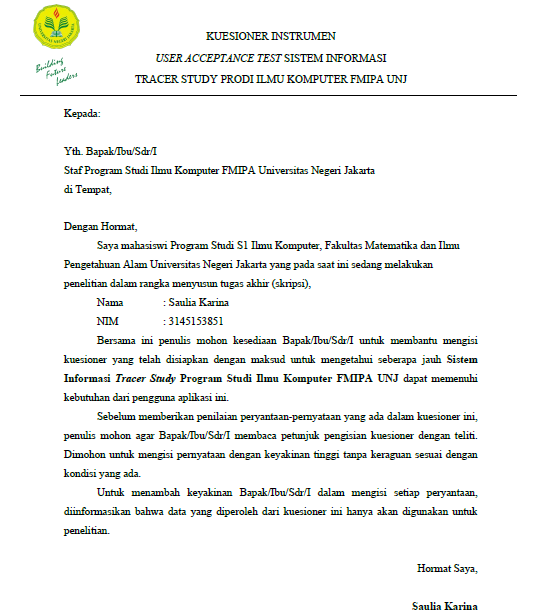
\includegraphics[width=15cm,height=18cm]{gambar/UAT/surat kuesioner}
	\label{surat_kuesioner}
\end{figure}

\begin{figure}[H]
	\centering
	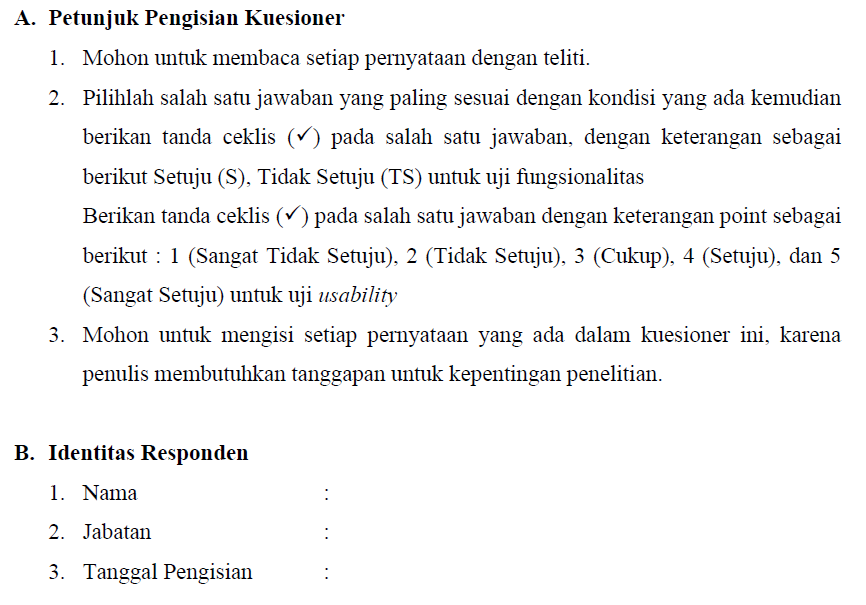
\includegraphics[width=10cm,height=12cm]{gambar/UAT/surat kuesioner 2}
	\label{surat_kuesioner2}
\end{figure}

\begin{figure}[H]
	\centering
	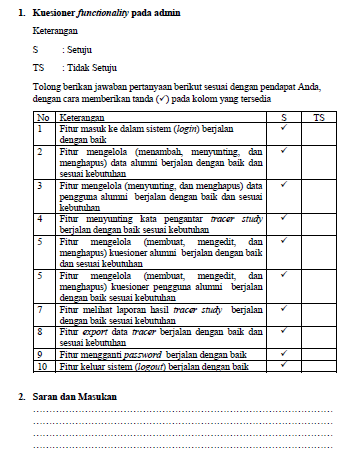
\includegraphics[width=15cm,height=18cm]{gambar/UAT/kf_admin}
	\label{kf_admin}
\end{figure}

\begin{figure}[H]
	\centering
	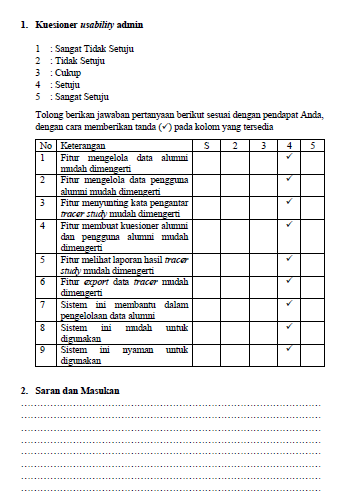
\includegraphics[width=15cm,height=18cm]{gambar/UAT/ku_admin}
	\label{ku_admin}
\end{figure}


\chapter{Kuesioner \textit{User Acceptance Test} pada Koorprodi}

\begin{figure}[H]
	\centering
	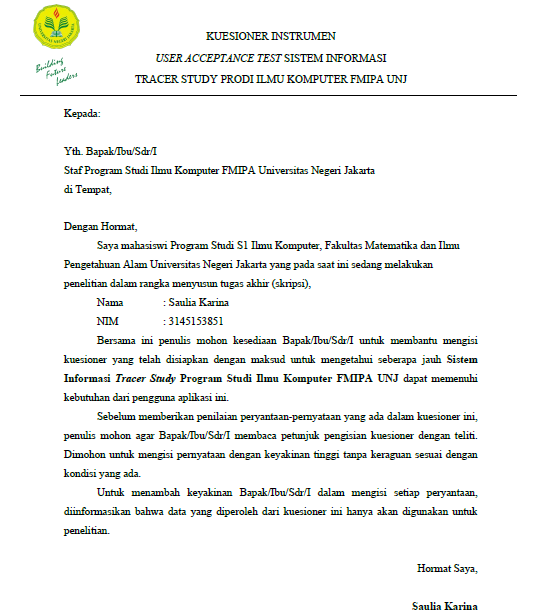
\includegraphics[width=15cm,height=18cm]{gambar/UAT/surat kuesioner}
	\label{surat_kuesioner}
\end{figure}

\begin{figure}[H]
	\centering
	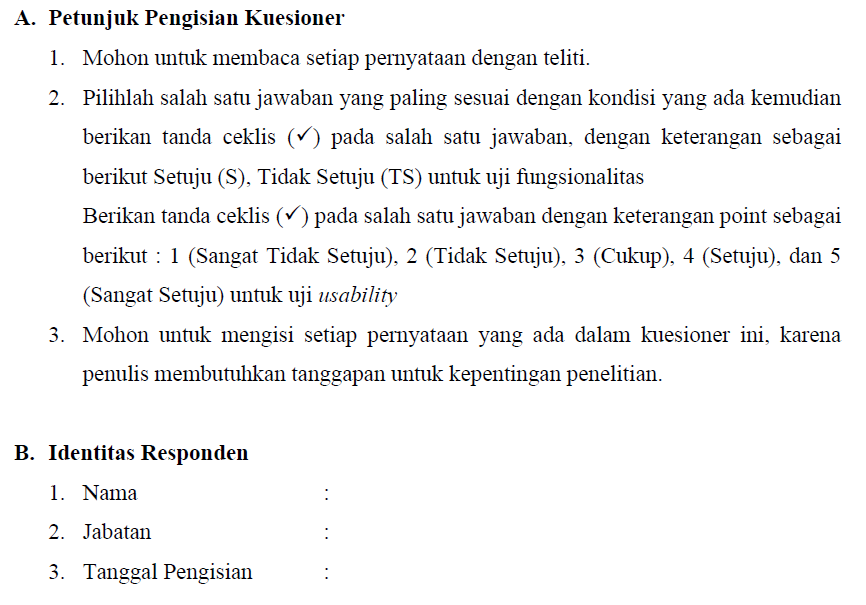
\includegraphics[width=10cm,height=12cm]{gambar/UAT/surat kuesioner 2}
	\label{surat_kuesioner2}
\end{figure}

\begin{figure}[H]
	\centering
	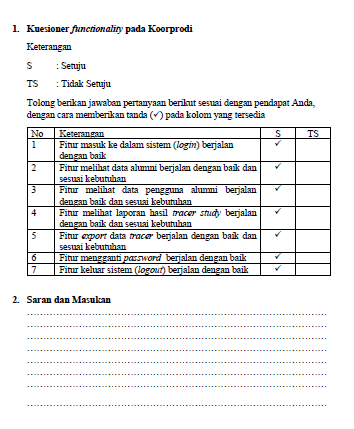
\includegraphics[width=15cm,height=18cm]{gambar/UAT/kf_koorprodi}
	\label{kf_koorprodi}
\end{figure}

\begin{figure}[H]
	\centering
	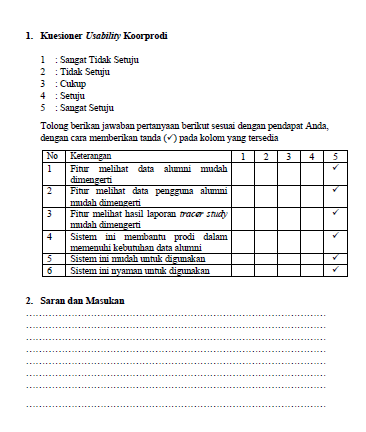
\includegraphics[width=15cm,height=18cm]{gambar/UAT/ku_koorprodi}
	\label{ku_koorprodi}
\end{figure}


\chapter{Kuesioner \textit{User Acceptance Test} pada Alumni}

\begin{figure}[H]
	\centering
	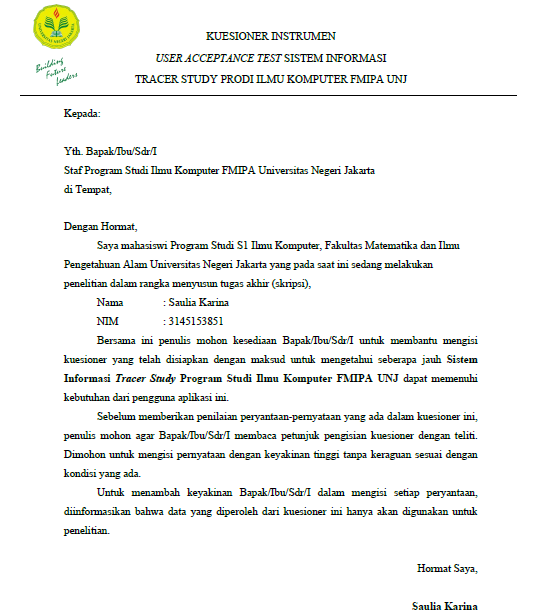
\includegraphics[width=15cm,height=18cm]{gambar/UAT/surat kuesioner}
	\label{surat_kuesioner}
\end{figure}

\begin{figure}[H]
	\centering
	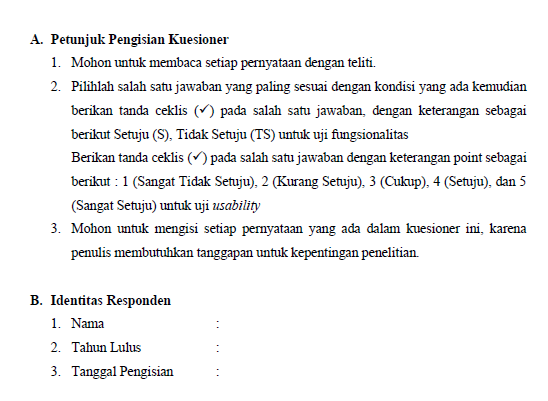
\includegraphics[width=10cm,height=12cm]{gambar/UAT/surat kuesioner 2 alumni}
	\label{surat_kuesioner2}
\end{figure}

\begin{figure}[H]
	\centering
	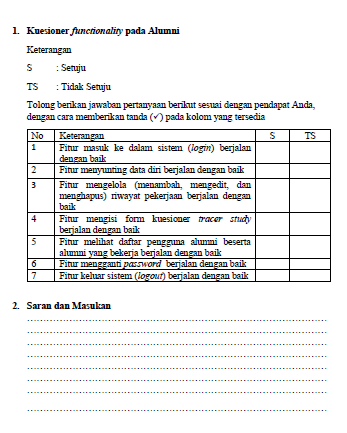
\includegraphics[width=15cm,height=18cm]{gambar/UAT/kf_alumni}
	\label{kf_alumni}
\end{figure}

\begin{figure}[H]
	\centering
	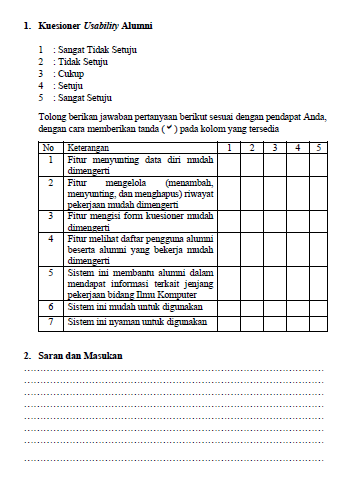
\includegraphics[width=15cm,height=18cm]{gambar/UAT/ku_alumni}
	\label{ku_alumni}
\end{figure}



\chapter{Kuesioner \textit{User Acceptance Test} pada Pengguna Alumni}

\begin{figure}[H]
	\centering
	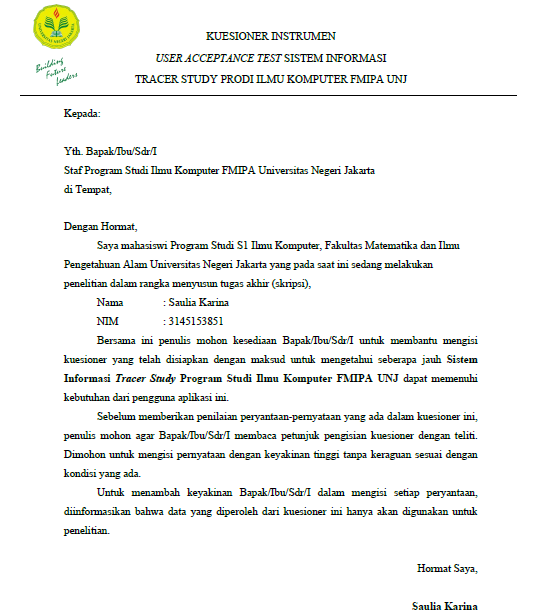
\includegraphics[width=15cm,height=18cm]{gambar/UAT/surat kuesioner}
	\label{surat_kuesioner}
\end{figure}

\begin{figure}[H]
	\centering
	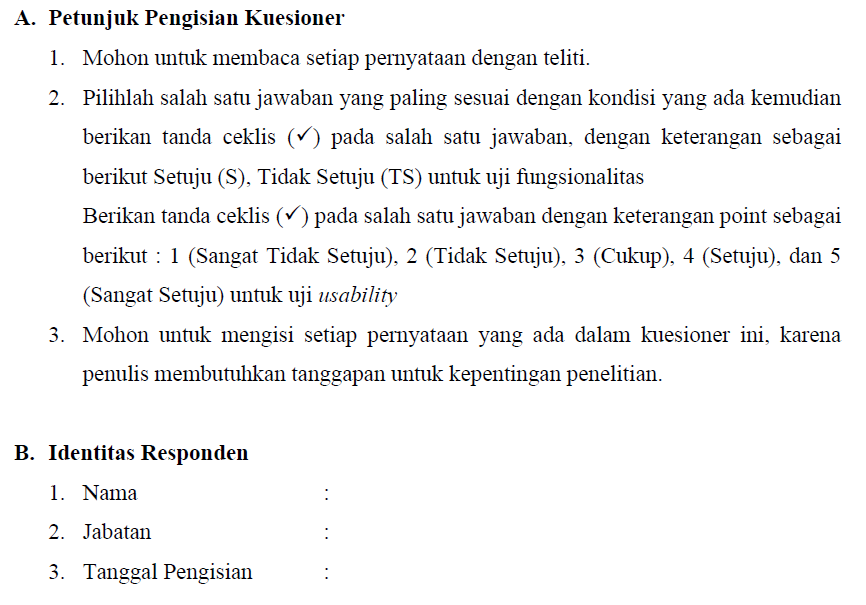
\includegraphics[width=10cm,height=12cm]{gambar/UAT/surat kuesioner 2}
	\label{surat_kuesioner2}
\end{figure}

\begin{figure}[H]
	\centering
	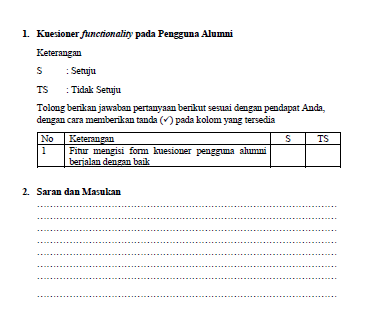
\includegraphics[width=15cm,height=18cm]{gambar/UAT/kf_pengguna}
	\label{kf_pengguna}
\end{figure}

\begin{figure}[H]
	\centering
	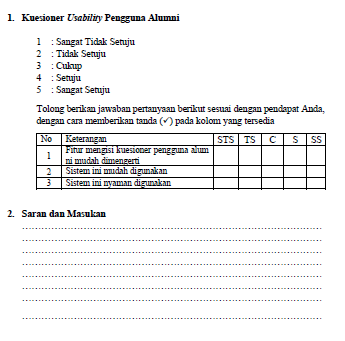
\includegraphics[width=15cm,height=18cm]{gambar/UAT/ku_pengguna}
	\label{ku_pengguna}
\end{figure}


\chapter{Kuesioner \textit{User Acceptance Test} pada Pengguna Alumni}